System zarządzania uczestnikami Sciencepreneurs Club stanowi przykład nowoczesnego podejścia do digitalizacji procesów organizacyjnych w środowisku akademickim. W świecie, gdzie efektywne zarządzanie danymi staje się kluczowym czynnikiem sukcesu inicjatyw edukacyjnych, implementacja zintegrowanych rozwiązań chmurowych nabiera szczególnego znaczenia. Rozdział ten prezentuje kompleksową analizę architektury systemu, który powstał jako odpowiedź na wyzwania związane z koordynacją cyklicznych wydarzeń klubu studenckiego.

Ten zautomatyzowany system opiera się na trzech kluczowych komponentach funkcjonalnych: \gls{forms}, \gls{powerautomate} oraz \gls{excel} wzbogacony o funkcjonalność \gls{powerquery}. Każdy z tych elementów, choć może funkcjonować niezależnie, w ramach opisywanego rozwiązania tworzy spójny łańcuch przetwarzania danych – od momentu rejestracji uczestnika, przez automatyzację przepływu informacji, aż po podstawową analizę danych frekwencji.

\section{Warstwa prezentacji - Microsoft Forms}

\gls{forms} to intuicyjna platforma do tworzenia formularzy i ankiet, które mogą być bezpośrednio powiązane z innymi narzędziami \gls{microsoft365}. W kontekście Sciencepreneurs Club, \gls{forms} pełni rolę frontendu całego systemu – jest pierwszym punktem kontaktu potencjalnego uczestnika. To właśnie za pomocą tego narzędzia realizowany jest proces rejestracji na poszczególne wydarzenia klubowe, stanowiąc cyfrową bramę wejściową do ekosystemu danych projektu.

Dostęp do formularzy jest ściśle kontrolowany poprzez hierarchiczny system uprawnień \cite{Microsoft365Groups2025}:

\begin{table}[ht]
\centering
\caption[Hierarchiczny system uprawnień do formularzy, źródło: dokumentacja Microsoft 365, omówienie grup dostępu dla administratorów \cite{Microsoft365Groups2025}]{Hierarchiczny system uprawnień do formularzy}
\renewcommand{\arraystretch}{1.3} % Zwiększenie odstępów między wierszami
\begin{tabular}{| >{\raggedright\arraybackslash}p{0.25\textwidth} | >{\raggedright\arraybackslash}p{0.65\textwidth} |}
\hline
\textbf{Poziom uprawnień} & \textbf{Zakres dostępu i możliwości} \\
\hline
Właściciele grupy (Group Owners) & Pełne uprawnienia administracyjne: tworzenie nowych formularzy, modyfikacja istniejących, zarządzanie dostępem innych użytkowników \\
\hline
Członkowie grupy (Group Members) & Przeglądanie i edytowanie formularzy z ograniczeniami dotyczącymi konfiguracji zaawansowanych ustawień bezpieczeństwa \\
\hline
Użytkownicy zewnętrzni & Ograniczony dostęp: wypełnianie formularzy bez możliwości dostępu do wyników lub ustawień (zależnie od konfiguracji formularza) \\
\hline
\end{tabular}
\vspace{0.5em}
\par\raggedright\footnotesize{Źródło: dokumentacja Microsoft 365, omówienie grup dostępu dla administratorów \cite{Microsoft365Groups2025}}
\end{table}

\gls{forms} oferuje wielopoziomowy system kontroli dostępu, który jest kluczowy dla zachowania integralności danych w środowisku akademickim. W implementacji dla Sciencepreneurs Club zastosowano model bezpieczeństwa oparty na grupach \gls{microsoft365}, gdzie wszystkie formularze są przechowywane w dedykowanej grupie \gls{inin}.

\gls{forms} implementuje kompleksowe mechanizmy ochrony danych, które stanowią istotny element strategii bezpieczeństwa informacji. Cała infrastruktura została zaprojektowana zgodnie z najwyższymi standardami branży \gls{it} zachowując zgodność z wymogami prawnymi oraz wielopoziomowe zabezpieczenia danych. 

\gls{forms} spełnia wymagania \gls{rodo} od momentu jego wejścia w życie w maju 2018 roku. Dodatkowo, platforma jest zgodna z ustawą \gls{hipaa} oraz umową \gls{baa}, co czyni ją odpowiednią do zastosowań w sektorach wrażliwych, takich jak ochrona zdrowia czy edukacja (zgodność z \gls{ferpa}). \cite{microsoft_forms_privacy_2024} Microsoft regularnie aktualizuje swoje rozwiązania w odpowiedzi na zmieniające się zagrożenia cybernetyczne oraz wymogi prawne, zapewniając stałą ochronę danych użytkowników przy jednoczesnym zachowaniu funkcjonalności i wygody korzystania z platformy.

Dane przechowywane na serwerach Microsoft są chronione na dwóch kluczowych poziomach \cite{microsoft_encryption_2024}:
\begin{itemize}
    \item \textbf{W czasie spoczynku} – wszystkie informacje zapisane na dyskach serwerów Microsoft podlegają szyfrowaniu. Oznacza to, że nawet w przypadku nieuprawnionego dostępu fizycznego do nośników, dane pozostają nieczytelne bez odpowiednich kluczy deszyfrujących.
    \item \textbf{Podczas tranzytu} – transmisja danych między użytkownikiem a serwerami (np. podczas wypełniania i przesyłania formularzy) jest zabezpieczona protokołem \gls{https}. Ta technologia efektywnie uniemożliwia przechwycenie informacji przez podmioty nieuprawnione podczas ich przesyłania przez sieć.
\end{itemize}

Istotną zaletą \gls{forms} w kontekście cyklicznych wydarzeń klubowych jest możliwość replikacji istniejących formularzy. Formularze z poprzednich edycji są zachowane nie tylko w celu archiwalnym, ale także jako szablon pod kolejne wydarzenia. Administrator w celu przygotowania nowej edycji kopiuje formularz z poprzedniej i uzupełnia informacje organizacyjne o najnowsze, takie jak numer edycji, prelegent, data, miejsce i temat spotkania. 

Po przygotowaniu formularza na kolejną edycję zostaje on opublikowany przez administratora. Uczestnicy za pomocą linku do formularza  wypełniają w nim kluczowe informacje zgłoszeniowe, takie jak imię i nazwisko, adres e-mail, zgoda na przetwarzanie danych oraz datę rejestracji.

Po pomyślnym wypełnieniu formularza, dane uczestnika są automatycznie przekazywane do dalszego przetwarzania poprzez integrację z \gls{powerautomate}, stanowiąc pierwszy etap zautomatyzowanego cyklu zarządzania danymi w ekosystemie Sciencepreneurs Club.

\section{Warstwa integracji - Power Automate}

\gls{powerautomate} (wcześniej Microsoft Flow) to narzędzie do tworzenia zautomatyzowanych przepływów pracy. W Sciencepreneurs Club pełni funkcję pośrednika między \gls{forms} a \gls{excel}. To właśnie w nim zakodowane jest automatyczne przekazywanie danych uczestników po wypełnieniu zgłoszenia do bazy danych „SC BAZA.xlsx”. 

\begin{figure}[!hb]
	\centering 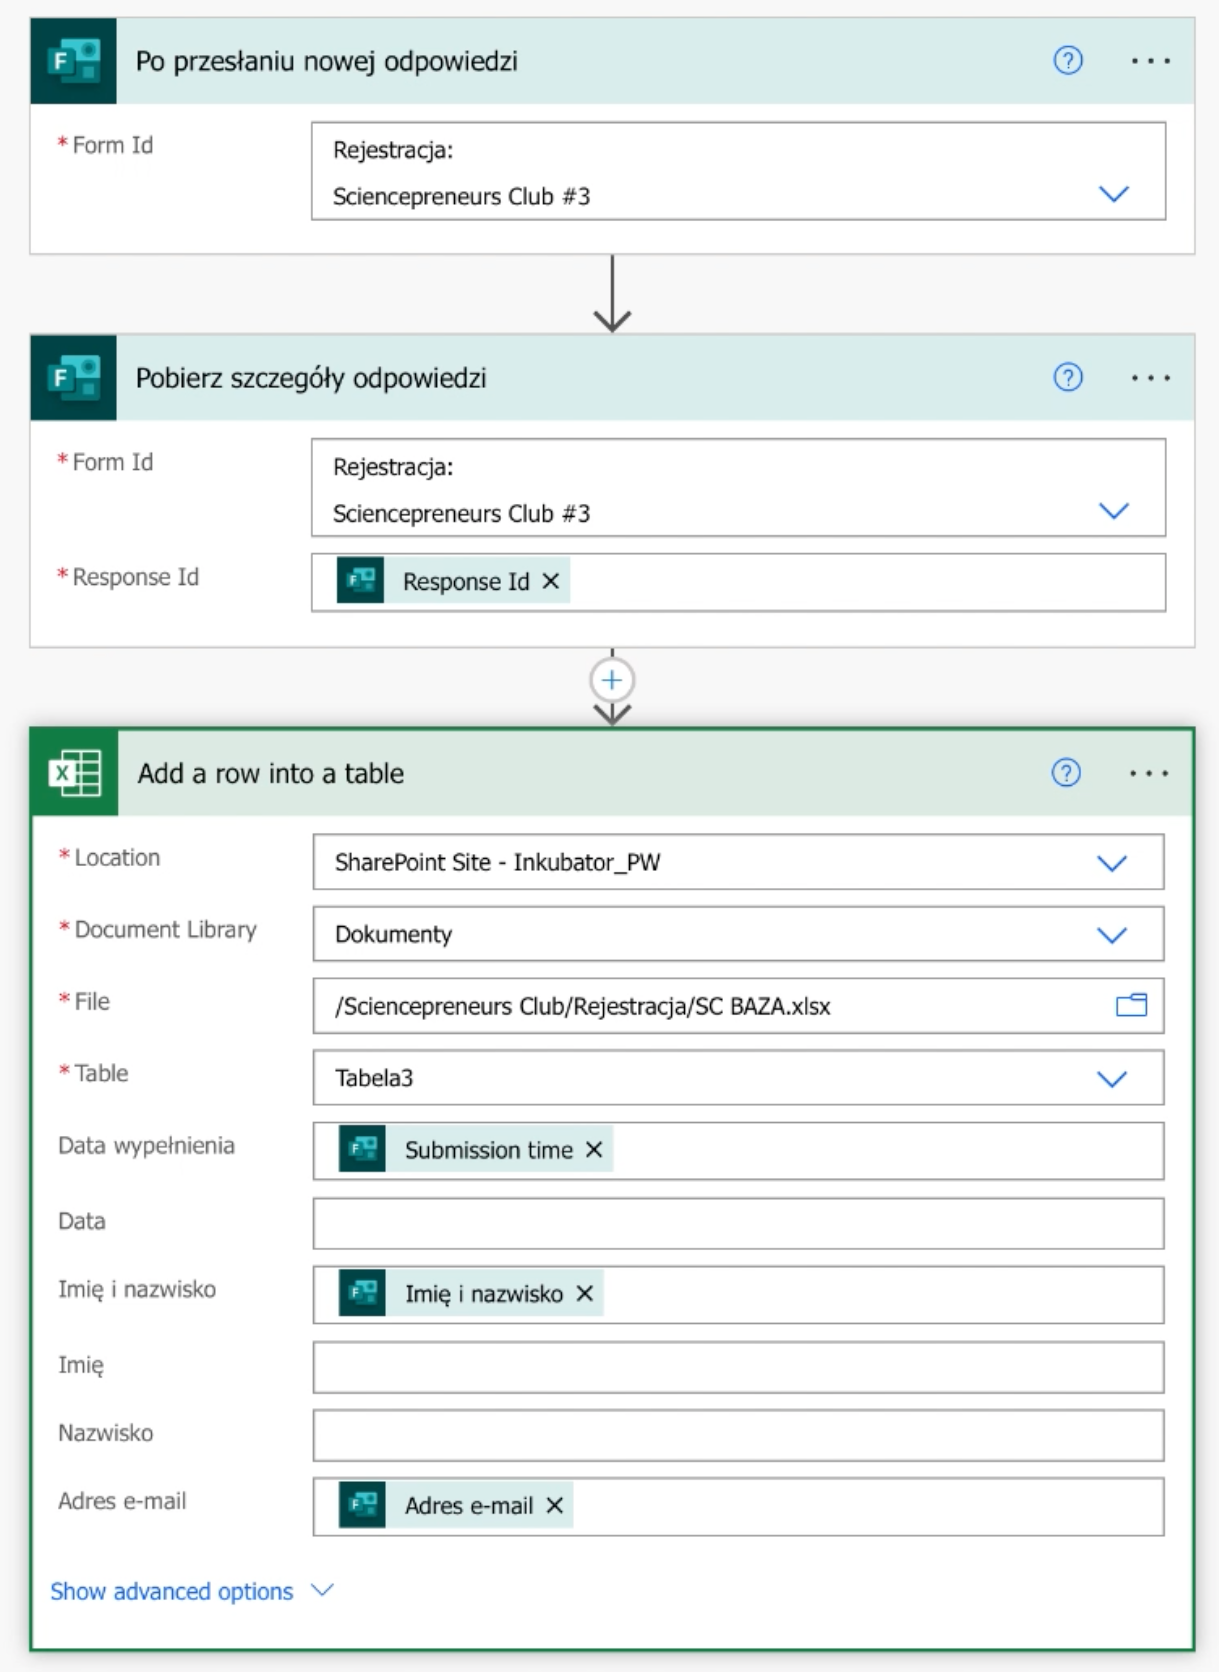
\includegraphics[width=0.7\linewidth]{rysunki/flow3.png}
	\caption{Power Automate Flow dla trzeciej edycji Sciencepreneurs Club, źródło: opracowanie własne }
\end{figure}

Dzieje się to poprzez poszczególne etapy przepływu pracy. 
Pierwszym z nich jest wyzwalacz. Każda nowa odpowiedź w Forms rozpoczyna działanie "Flow", gdy uczestnik wypełni formularz rejestracyjny. Aktywacja przepływu następuje automatycznie w momencie złożenia nowego zgłoszenia w formularzu \gls{forms}. \cite{microsoft_power_automate_2025} Wyzwalacz \gls{powerautomate} funkcjonuje na zasadzie nasłuchiwania określonych zdarzeń w połączonych aplikacjach. W przypadku Sciencepreneurs Club, wyzwalacz jest skonfigurowany do monitorowania konkretnego formularza \gls{forms}, zidentyfikowanego przez unikalny identyfikator widoczny w polu "Form Id". Jednak nie ma potrzeby kopiowania ID formularza, narzędzie zostało przygotowane w ten sposób, że wystarczy wybrać odpowiednią nazwę z listy, jak na rysunku 7.1. Poprawne powiązanie Flow z formularzem jest absolutnie kluczowe dla funkcjonowania całego systemu - każda zmiana formularza wymaga aktualizacji tego identyfikatora, co jest realizowane podczas przygotowywania nowej edycji wydarzenia.

\begin{figure}[!hb]
	\centering 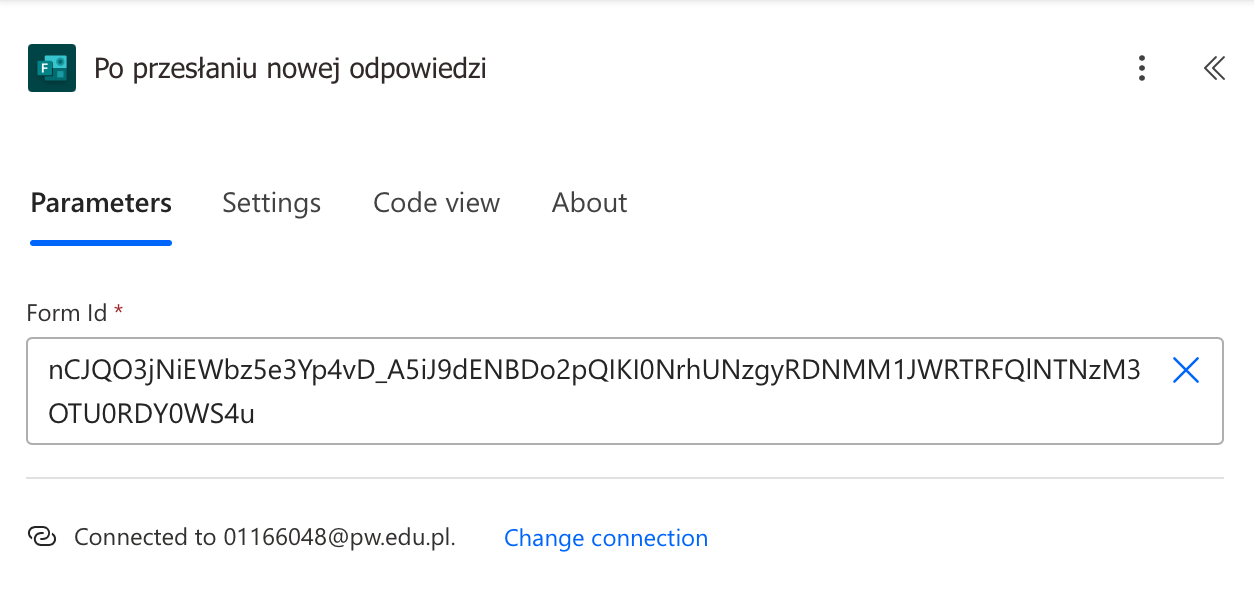
\includegraphics[width=0.7\linewidth]{rysunki/KonfiguracjaPowerAutomate.png}
	\caption{Konfiguracja wyzwalacza Power Automate Flow, źródło: opracowanie własne z użyciem narzędzia \gls{powerautomate}}
\end{figure}

Na rysunku 7.2. widać, że system jest skonfigurowany w kontekście konta uczelnianego \gls{pw} (01166048@pw.edu.pl). Jest to fundamentalny element architektury systemu, gdyż umożliwia za pomocą grup dostępu bezpośrednie połączenie do grupy Inkubator\_PW należącej do \gls{inin}. To połączenie gwarantuje dostęp do zasobów przechowywanych w \gls{onedrive} \gls{pw} oraz zachowanie ciągłości dostępu dla kolejnych administratorów systemu w ramach uczelni.

Istotnym aspektem architektury \gls{powerautomate}, który warto podkreślić, jest sposób, w jaki graficzny interfejs użytkownika współpracuje z kodem JSON stanowiącym podstawę funkcjonowania przepływów. W kontekście systemu Sciencepreneurs Club, administrator konfigurujący przepływ nie musi bezpośrednio pisać kodu. Proces konfiguracji wyzwalacza dla formularza \gls{forms} przebiega następująco:

\begin{itemize}
    \item Administrator wybiera typ wyzwalacza "Po przesłaniu nowej odpowiedzi" z galerii dostępnych wyzwalaczy Microsoft Forms.
    \item Następnie, z rozwijanej listy dostępnych formularzy, wskazuje konkretny formularz rejestracyjny dla danej edycji Sciencepreneurs Club.
    \item Power Automate automatycznie pobiera unikalny identyfikator formularza i generuje odpowiedni kod JSON w tle.
\end{itemize}

To, co widzimy w prezentowanym kodzie JSON, jest faktycznie efektem tych działań w interfejsie, a nie kodem napisanym ręcznie przez administratora. Platforma \gls{powerautomate} przetwarza wybory dokonane w interfejsie graficznym na strukturalną definicję przepływu w formacie JSON, która następnie jest interpretowana przez \gls{flowengine} pracy platformy.\cite{microsoft_power_automate_2025} W przypadku Sciencepreneurs Club, przepływ to cała sekwencja automatyzacji od momentu wypełnienia formularza przez uczestnika, przez zapisanie jego danych w \gls{excel}.

\begin{lstlisting}[language=JSON, caption=Konfiguracja wyzwalacza Power Automate w języku JSON źródło: kod wygenerowany na podstwie konfiguracji poprzez narzędzie Power Automate]
{
  "type": "OpenApiConnectionWebhook",
  "inputs": {
    "parameters": {
      "form_id": "nCJQO3jNiEWbz5e3Yp4vD_A5iJ9dENBDo2pQIKI0NrhUNzgyRDNMM1JWRTR
      FQlNTNzM3OTU0RDY0WS4u"
    },
    "host": {
      "apiId": "/providers/Microsoft.PowerApps/apis/shared_microsoftforms",
      "connection": "shared_microsoftforms",
      "operationId": "CreateFormWebhook"
    }
  },
  "splitOn": "@triggerOutputs()?['body/value']",
  "metadata": {
    "operationMetadataId": "c82c4e1e-d1d3-4721-a97a-27e2155adc56"
  }
}
\end{lstlisting}

Przedstawiony fragment kodu JSON  7.1. definiuje szczegółową konfigurację wyzwalacza. Choć ten kod nie jest pisany ręcznie przez administratora, zrozumienie jego struktury pozwala lepiej pojąć, jak działa automatyzacja w systemie.

Fragment kodu rozpoczyna się określeniem typu wyzwalacza jako \texttt{"OpenApiConnectionWebhook"}. Oznacza to, że nasz wyzwalacz wykorzystuje standardowy sposób komunikacji między usługami \gls{microsoft365}, działając jak cyfrowy czujnik nasłuchujący określonych wydarzeń.

W sekcji \texttt{"inputs"} znajdują się wszystkie informacje wejściowe potrzebne do prawidłowego działania wyzwalacza. Najważniejszym elementem jest parametr \texttt{"form\_id"}, który zawiera długi ciąg znaków jednoznacznie identyfikujący formularz \gls{forms}, który ma być monitorowany. To właśnie ten identyfikator wiąże nasz przepływ z konkretnym formularzem rejestracyjnym wydarzenia.

Dalej w kodzie znajduje się sekcja \texttt{"host"}, która określa, z jakim systemem nasz wyzwalacz będzie się komunikował. Parametr \texttt{"apiId"} wskazuje, że będziemy korzystać z \gls{api} \gls{forms}, a \texttt{"connection"} określa typ połączenia jako standardowe połączenie do \gls{forms}. Parametr \texttt{"operationId"} precyzuje, że konkretna operacja to \texttt{"CreateFormWebhook"}, czyli utworzenie mechanizmu nasłuchującego nowych odpowiedzi w formularzu.

Kolejny element, \texttt{"splitOn"} definiuje sposób, w jaki dane z formularza będą przetwarzane przez przepływ. Ta techniczna instrukcja informuje silnik przepływów, jak ma rozdzielać otrzymane odpowiedzi na poszczególne elementy danych, które będą wykorzystywane w dalszych krokach przepływu.

Na końcu znajduje się sekcja \texttt{"metadata"} zawierająca unikalny identyfikator operacji. Jest to wewnętrzny znacznik używany przez \gls{powerautomate} do śledzenia i zarządzania przepływem podczas jego wykonywania.

Wszystkie te elementy razem tworzą kompletną definicję wyzwalacza. Gdy tylko pojawi się nowa odpowiedź, wyzwalacz aktywuje się i uruchamia pozostałe kroki przepływu.

Kolejnym krokiem jest pobranie danych, \gls{powerautomate} pobiera szczegóły odpowiedzi wprowadzone przez uczestnika, wraz z metadanymi formularza i przekazuje je do \gls{excel}. Ponownie jak w pierwszym kroku wyzawalacza, należy skonfigurować do monitorowania konkretnego formularza Microsoft Forms. W tym przypadku jest to ten sam formularz (to samo ID). 

\begin{lstlisting}[language=JSON, caption=Konfiguracja pobrania szczegółów odpowiedzi z formularza w Power Automate w języku JSON źródło: kod wygenerowany na podstwie konfiguracji poprzez narzędzie Power Automate]
{
  "type": "OpenApiConnection",
  "inputs": {
    "parameters": {
      "form_id": "nCJQO3jNiEWbz5e3Yp4vD_A5iJ9dENBDo2pQIKI0NrhUNzgyRDNMM1JWRTR
      FQlNTNzM3OTU0RDY0WS4u",
      "response_id": "@triggerOutputs()?['body/resourceData/responseId']"
    },
    "host": {
      "apiId": "/providers/Microsoft.PowerApps/apis/shared_microsoftforms",
      "connection": "shared_microsoftforms",
      "operationId": "GetFormResponseById"
    }
  },
  "runAfter": {},
  "metadata": {
    "operationMetadataId": "f2fea26e-bc97-4c91-8a2b-9dc2c7fb6e4f"
  }
}
\end{lstlisting}

Podczas gdy pierwszy kod 7.1.(wyzwalacz) informował system, aby nasłuchiwał nowych odpowiedzi w formularzu, ten kod 7.2. określa, co należy zrobić, gdy taka odpowiedź się pojawi.

Typ tego kroku to \texttt{"OpenApiConnection"}, co oznacza standardowe połączenie z usługą \gls{microsoft365}. W przeciwieństwie do poprzedniego kroku, który był typu \texttt{"OpenApiConnectionWebhook"}, ten krok nie nasłuchuje zdarzeń, ale aktywnie pobiera dane.

W sekcji \texttt{"inputs"} znajdują się parametry potrzebne do pobrania szczegółowych informacji o odpowiedzi na formularz. Widzimy tu dwa ważne elementy. Pierwszy \texttt{"form\_id"} - ten sam identyfikator formularza co w poprzednim kroku, który wskazuje, z którego formularza mamy pobrać dane. Oraz \texttt{"response\_id"} - tutaj pojawia się: \texttt{"@triggerOutputs()}\texttt{['body/resourceData} \texttt{/responseId']}. Ta dynamiczna wartość pobiera identyfikator konkretnej odpowiedzi z danych wyzwalacza. Innymi słowy, system pobiera identyfikator nowo złożonego zgłoszenia, aby następnie pobrać jego szczegóły.

W sekcji \texttt{"host"} widzimy podobne informacje jak wcześniej - używamy \gls{api} \gls{forms}, ale tym razem operacja to \texttt{"GetFormResponseById"}. Nazwa ta jasno wskazuje cel: pobranie szczegółów odpowiedzi na podstawie jej identyfikatora.

Element \verb|"runAfter": {}| informuje system, że ten krok powinien zostać wykonany bezpośrednio po uruchomieniu wyzwalacza, bez żadnych dodatkowych warunków czy opóźnień.

Na koniec mamy sekcję \texttt{"metadata"} z unikalnym identyfikatorem operacji, który służy do wewnętrznego zarządzania tym krokiem w \gls{powerautomate}. Pobiera wszystkie szczegółowe informacje z formularza, gdy ktoś go wypełni. Te dane będą następnie dostępne dla kolejnych kroków przepływu.

Finalnym etapem naszego zautomatyzowanego przepływu jest zapisanie danych uczestnika w arkuszu \gls{excel} w dopasowanej kolumnie, który służy jako centralna baza danych Sciencepreneurs Club. W ten sposób każda wypełniona w \gls{forms} ankieta jest automatycznie eksportowana do pliku \gls{excel}, gdzie stanowi punkt wyjścia do dalszego przetwarzania danych. Ten krok zamyka pętlę procesu, zapewniając, że informacje wprowadzone przez uczestnika w formularzu \gls{forms} zostaną trwale przechowane i będą dostępne do dalszej analizy.

\begin{figure}[!hb]
	\centering 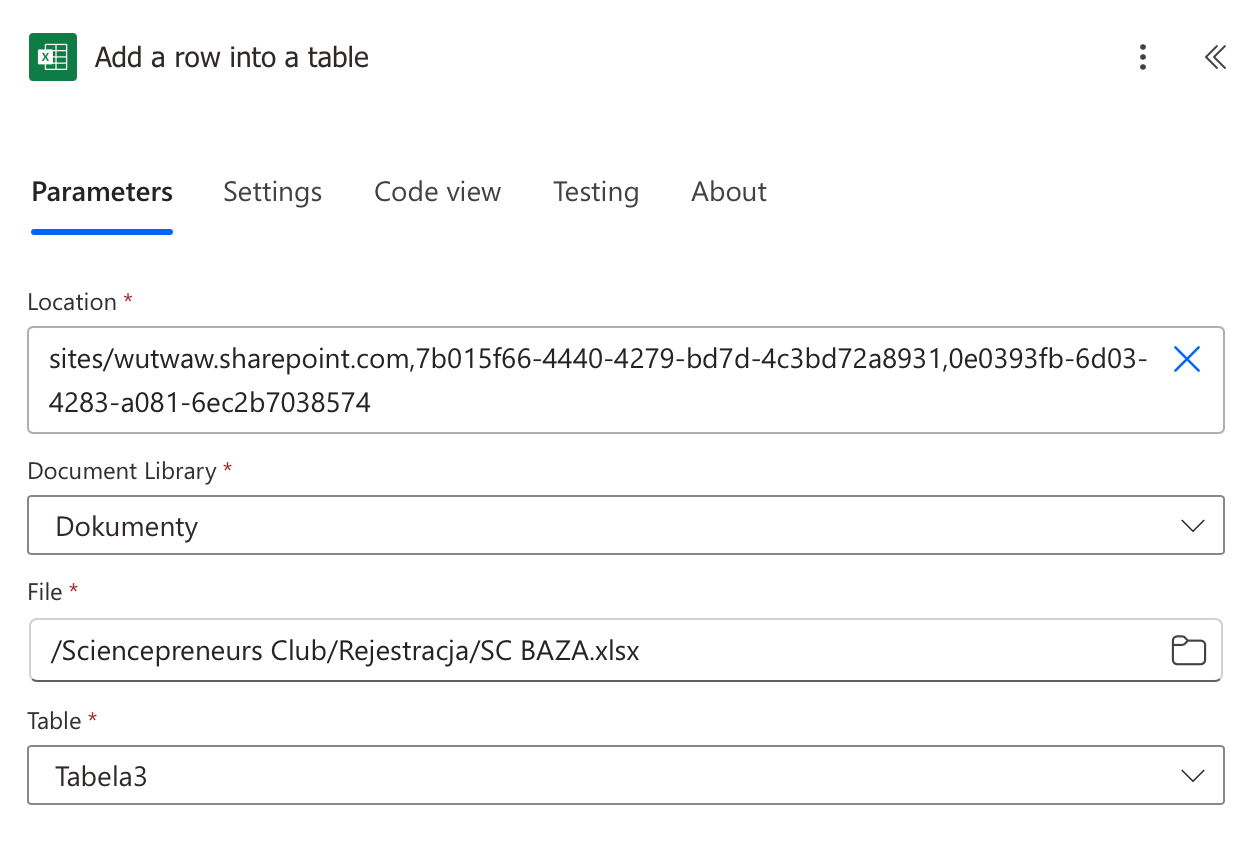
\includegraphics[width=0.7\linewidth]{rysunki/DodanieWiersza.png}
	\caption{Podstwowe parametry konfiguracji ładowania danych do nowego wiersza Microsoft Excel z użyciem Power Automate Flow, źródło: opracowanie własne z użyciem narzędzia \gls{powerautomate}}
\end{figure}

Administrator musi zdefiniować kluczowe parametry. Te wizualne wybory są następnie przekształcane przez system w precyzyjne identyfikatory w kodzie konfiguracyjnym, zapewniając jednoznaczne wskazanie miejsca docelowego dla danych uczestników. Parametry te definiują ścieżkę, którą podążą dane z formularza, aby finalnie trafić do odpowiedniego arkusza w pliku \gls{excel} przechowywanym w środowisku chmurowym \gls{microsoft365}.

W tym samym kroku administrator definiuje, które pola z formularza (identyfikowane przez unikalne identyfikatory odpowiedzi) mają zostać zapisane w jakich kolumnach tabeli \gls{excel}. Interfejs \gls{powerautomate} umożliwia wybór dynamicznych wartości z wcześniejszego kroku \texttt{"Pobierz\_szczegóły\_odpowiedzi"}.

\newpage
\begin{figure}[!hb]
	\centering 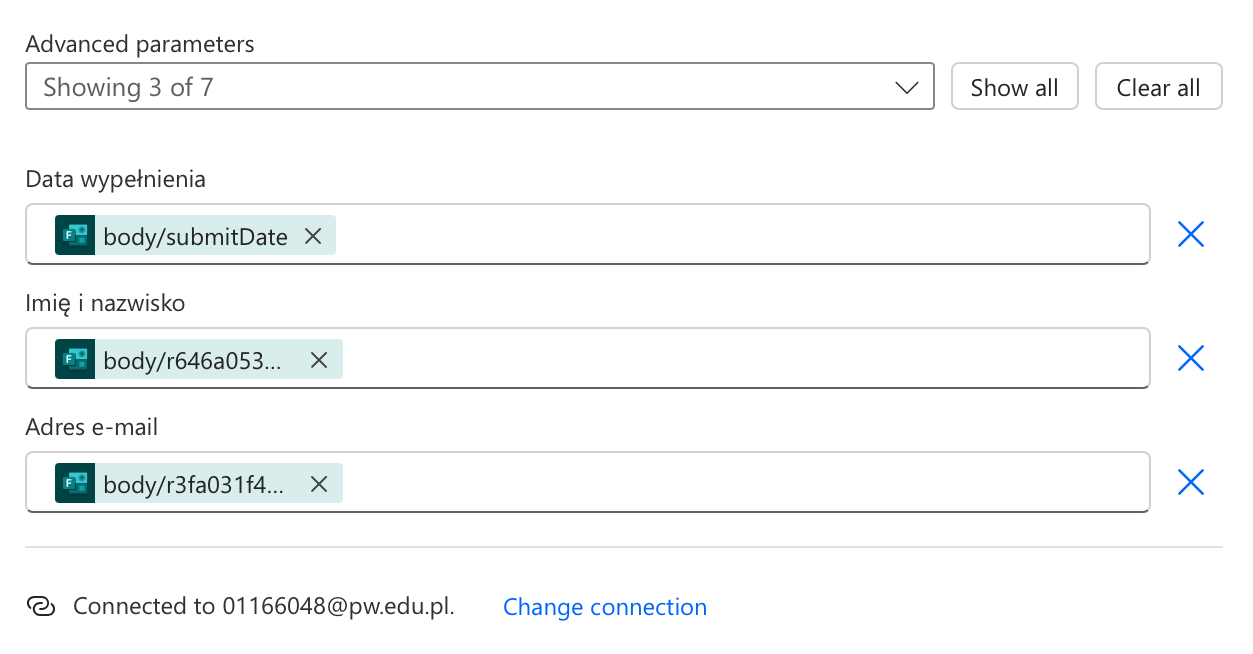
\includegraphics[width=0.7\linewidth]{rysunki/DodanieWierszaAdvanced.png}
	\caption{Zaawansowane parametry konfiguracji ładowania danych do nowego wiersza Microsoft Excel z użyciem Power Automate Flow, źródło: opracowanie własne z użyciem narzędzia \gls{powerautomate}}
\end{figure}

Cały ten proces jest zakodowany w przedstawionym poniżej fragmencie konfiguracji JSON, który został automatycznie wygenerowany na podstawie wizualnych wyborów administratora w interfejsie \gls{powerautomate}. 

\begin{lstlisting}[language=json, caption={Konfiguracja przesyłu danych uczestników do Microsoft Excel z użyciem Power Automate w języku JSON źródło: kod wygenerowany na podstwie konfiguracji poprzez narzędzie Power Automate}]
{
  "type": "OpenApiConnection",
  "inputs": {
    "parameters": {
      "source": "sites/wutwaw.sharepoint.com,7b015f66-4440-4279-bd7d-4c3bd72
      a8931,0e0393fb-6d03-4283-a081-6ec2b7038574",
      "drive": "b!Zl8Be0BEeUK9fUw71yqJMfuTAw4DbYNCoIFuwrcDhXTgMT7sGhSoQ5bE7
      X0hmj-I",
      "file": "01LCUGMVPW6OFHMRQPFVCLYQOK2IH7ACRI",
      "table": "{F5EC12A3-50AA-41BF-834D-21E3EA8E22A8}",
      "item/Data wypelnienia": "@outputs('Pobierz_szczegoly_odpowiedzi')?
      ['body/submitDate']",
      "item/Imie i nazwisko": "@outputs('Pobierz_szczegoly_odpowiedzi')?
      ['body/r646a053d893e4a02be72a3f3150f89be']",
      "item/Adres e-mail": "@outputs('Pobierz_szczegoly_odpowiedzi')?
      ['body/r3fa031f484ed42afb455515c030b4054']"
    },
    "host": {
      "apiId": "/providers/Microsoft.PowerApps/apis/shared_excelonlinebusin
      ess",
      "connection": "shared_excelonlinebusiness-1",
      "operationId": "AddRowV2"
    }
  },
  "runAfter": {
    "Pobierz_szczegoly_odpowiedzi": [
      "Succeeded"
    ]
  },
  "metadata": {
    "01LCUGMVPW6OFHMRQPFVCLYQOK2IH7ACRI": "/Sciencepreneurs Club/Rejestracja/SC BAZA.xlsx",
    "operationMetadataId": "32bed134-874d-48d6-9a14-1e98fdbd233f",
    "tableId": "{F5EC12A3-50AA-41BF-834D-21E3EA8E22A8}"
  }
}
\end{lstlisting}

Przedstawiony fragment kodu określa, w jaki sposób dane z formularza zostaną zapisane w arkuszu \gls{excel}. Typ tego kroku to \texttt{"OpenApiConnection"}, co oznacza standardowe połączenie z usługą \gls{microsoft365}, w tym przypadku z \gls{excel} Online.

W sekcji \texttt{"inputs"} znajdujemy szereg parametrów, które są niezbędne do precyzyjnego zapisania danych. 

Parametr \texttt{"source"} zawiera identyfikator lokalizacji w \gls{sharepoint}, gdzie przechowywany jest plik \gls{excel}. Ten długi ciąg znaków jednoznacznie wskazuje na witrynę \gls{sharepoint} \gls{pw} (wutwaw.sharepoint.com), a kolejne identyfikatory określają dokładną lokalizację w strukturze folderów. 

Parametr \texttt{"drive"} identyfikuje konkretny dysk w \gls{sharepoint}, gdzie znajduje się nasz plik, a \texttt{"file"} wskazuje dokładnie na plik \gls{excel} o nazwie \texttt{"SC BAZA.xlsx"}, co widzimy w sekcji metadanych.

Parametr \texttt{"table"} zawiera unikalny identyfikator tabeli w arkuszu \gls{excel}, do której będziemy dodawać nowy wiersz z danymi uczestnika.
Następnie widzimy serię parametrów definiujących wartości, które zostaną zapisane w poszczególnych kolumnach tabeli. \texttt{"item/Data wypełnienia"} pobiera datę złożenia formularza z poprzedniego kroku \texttt{"item/Imię i nazwisko"} pobiera imię i nazwisko uczestnika \texttt{"item/Adres e-mail"} pobiera adres e-mail. 

Każda z tych wartości jest pobierana z  poprzedniego kroku \texttt{Pobierz\_szczegóły\_odpowiedzi} przy użyciu wyrażenia rozpoczynającego się od \texttt{@outputs}. Wyrażenia te odwołują się do konkretnych pól formularza po ich unikalnych identyfikatorach.

W sekcji \texttt{"host"} widzimy, że używamy \gls{api} Excel Online Business, a operacja to \texttt{"AddRowV2"}, co jednoznacznie wskazuje, że dodajemy nowy wiersz do tabeli.

Element \texttt{"runAfter"} określa, że ten krok zostanie wykonany tylko po pomyślnym zakończeniu kroku \texttt{"Pobierz\_szczegóły\_odpowiedzi"}. Jest to logiczne zabezpieczenie - system najpierw musi pobrać dane z formularza, zanim będzie mógł je zapisać w Excelu.

Sekcja \texttt{"metadata"} zawiera dodatkowe informacje, w tym ścieżkę do pliku \gls{excel} \texttt{"/Sciencepreneurs Club/Rejestracja/SC BAZA.xlsx"} oraz identyfikatory używane przez system do śledzenia operacji.

Warto zauważyć, że choć kod zawiera wiele technicznych szczegółów, administrator tworzy ten krok w prosty sposób - wybierając akcję \texttt{"Add a row into a table"} w \gls{excel}, wskazując lokalizację pliku i tabeli, a następnie mapując pola formularza do odpowiednich kolumn w tabeli. \gls{powerautomate} automatycznie generuje cały ten kod na podstawie wizualnych wyborów użytkownika.

Po wykonaniu tego kroku, dane uczestnika są bezpiecznie zapisane w bazie \gls{excel}, gotowe do dalszego wykorzystania przez zespół organizacyjny Sciencepreneurs Club. Dzięki temu zautomatyzowanemu procesowi, administrator nie musi ręcznie eksportować danych z \gls{forms} do \gls{excel}, eliminując potencjalne błędy ludzkie i oszczędzając cenny czas.


\section{Warstwa danych i analizy - Microsoft Excel z Power Query}

\gls{excel} jako narzędzie do przechowywania i analizy danych w systemie Sciencepreneurs Club stanowi rozwiązanie będące kompromisem między praktycznością a optymalnymi praktykami zarządzania danymi. Wybór ten, choć niepozbawiony ograniczeń technicznych, odzwierciedla realia organizacyjne i zasobowe \gls{inin}, gdzie priorytetem było szybkie wdrożenie systemu w ramach istniejącej infrastruktury \gls{microsoft365}.

Plik \gls{excel} \texttt{"SC BAZA.xlsx”} pełni rolę centralnej bazy danych, w której przechowywane są informacje o wszystkich uczestnikach programu. Znajduje się on na \gls{onedrive} \gls{pw} na kanale \gls{inin} \texttt{"Inkubator\_PW"} w folderze Sciencepreneurs Club. Składa się z kilku kluczowych arkuszy:

\begin{itemize}
    \item \textbf{Baza (unikatowi uczestnicy)} – lista unikalnych uczestników i liczba edycji, w których wzięli udział.
    \item \textbf{Baza} – główna lista wszystkich rejestracji uczestników w poszczególnych edycjach.
    \item \textbf{Uczestnicy \#1, Uczestnicy \#2, Uczestnicy \#3} – arkusze dedykowane każdej edycji Sciencepreneurs Club. Z każdą nową edycją liczba arkuszy będzie rosła analogicznie. Dzięki temu dane z poszczególnych edycji są łatwo dostępne. To do tych arkuszy trafiają dane zebrane z rejestracji online za pomocą formularza \gls{forms}. 
\end{itemize}

Przy analizie warstwy danych i analizy wykorzystującej \gls{excel} z \gls{powerquery} w systemie Sciencepreneurs Club, istotnym elementem jest omówienie aspektów bezpieczeństwa i zarządzania dostępem. 

Wybór \gls{excel} jako głównej bazy danych, choć uzasadniony w kontekście organizacyjnym, niesie jednak ze sobą szereg ograniczeń i wyzwań, które należy świadomie adresować.

\begin{itemize}
\item \textbf{Granularność uprawnień} – Excel nie pozwala na definiowanie uprawnień na poziomie poszczególnych rekordów czy kolumn. Dostęp jest kontrolowany na poziomie całego pliku lub, w ograniczonym zakresie, na poziomie arkuszy poprzez ich blokowanie. \cite{microsoft_excel_blocking_2025}
\item \textbf{Śledzenie zmian} – choć \gls{onedrive}/\gls{sharepoint} oferuje historię wersji, nie dorównuje ona funkcjonalności integralności referencyjnej (każda wartość klucza obcego w jednej tabeli odnosi się do istniejącego rekordu w tabeli nadrzędnej) ani transakcyjnej, co oznacza, że użytkownicy mogą wprowadzać niespójne dane, dostępnych w systemach \gls{sql}, co utrudnia audyt zmian. \cite{microsoft_office_versions_2025}
\item \textbf{Ryzyko nieautoryzowanych modyfikacji} – każdy użytkownik z uprawnieniami edycji może potencjalnie zmodyfikować nie tylko dane, ale również strukturę arkuszy czy formuły \gls{powerquery}, co stanowi istotne ryzyko dla integralności danych. \cite{Microsoft365Groups2025}
\item \textbf{Brak walidacji na poziomie komórek} – \gls{excel} nie oferuje równie zaawansowanych mechanizmów walidacji jak systemy \gls{dbms}, co zwiększa ryzyko wprowadzenia niepoprawnych lub niespójnych danych. \cite{microsoft_excel_validation_2025}
\end{itemize}

W systemie Sciencepreneurs Club ograniczenia te są częściowo kompensowane przez warstwę kontroli dostępu oferowaną przez platformę \gls{sharepoint}, gdzie plik jest przechowywany. Dostęp do pliku jest limitowany do członków grupy \gls{inin}, co stanowi pierwszą linię obrony przed nieautoryzowanym dostępem.

Plik \gls{excel} \texttt{"SC BAZA.xlsx"} przechowywany na \gls{onedrive} \gls{pw} w folderze Sciencepreneurs Club na kanale \gls{inin} \texttt{"Inkubator\_PW"} dzięki zaawansowanym standardom bezpieczeństwa \gls{microsoft365} podlega wielopoziomowemu systemowi zabezpieczeń. \cite{Microsoft365Groups2025}

\begin{itemize}
    \item \textbf{Brak dostępu zewnętrznego} - w obecnej konfiguracji plik nie jest udostępniany użytkownikom spoza domeny \gls{pw}. \cite{Microsoft365Groups2025}
    \item \textbf{Uwierzytelnianie dwuskładnikowe} - dostęp do pliku wymaga logowania do konta \gls{pw}, które może być dodatkowo zabezpieczone przez uwierzytelnianie dwuskładnikowe. \cite{kastwal2023}
    \item \textbf{Kontrola dostępu na poziomie \gls{sharepoint}/\gls{onedrive}} - dostęp do pliku jest ograniczony do członków grupy \gls{inin} oraz administratorów platformy. Uprawnienia są dziedziczone z nadrzędnej struktury folderów, zapewniając spójny model bezpieczeństwa. \cite{Microsoft365Groups2025}
    \item \textbf{Historia wersji} - \gls{onedrive} automatycznie przechowuje wcześniejsze wersje dokumentu, umożliwiając odzyskanie danych w przypadku nieautoryzowanych zmian lub uszkodzenia pliku. \cite{microsoft_office_versions_2025}
\end{itemize}

Excel jako narzędzie do przechowywania danych posiada pewne ograniczenia wydajnościowe, które teoretycznie mogłyby wpływać na funkcjonowanie systemu. \gls{excel}posiada ograniczenie limitów pojemności do 1 048 576 wierszy na arkusz.\cite{microsoft_excel_specs_2025} Złożone transformacje \gls{powerquery} mogą wpływać na wydajność, responsywność pliku.

W kontekście Sciencepreneurs Club, prawdopodobieństwo przekroczenia tych limitów jest jednak znikome. Biorąc pod uwagę skalę wydarzenia (kilkadziesiąt do maksymalnie kilkuset uczestników per edycja) oraz częstotliwość organizacji (kilka edycji rocznie), system mógłby funkcjonować przez wiele lat bez zbliżania się do technicznych ograniczeń \gls{excel}. Nawet przy ambitnym założeniu rozwoju inicjatywy, liczba zapisów w bazie prawdopodobnie nie przekroczyłaby kilkudziesięciu tysięcy w perspektywie długoterminowej, co stanowi zaledwie ułamek możliwości \gls{excel}.

Dlatego, choć świadomość tych ograniczeń jest istotna z perspektywy projektowej, nie stanowią one realnego zagrożenia dla funkcjonalności systemu w przewidywalnej przyszłości.

\gls{powerquery} pełni w systemie rolę zbliżoną do silnika zapytań w tradycyjnych bazach danych, umożliwiając transformację, filtrowanie i agregację danych bez konieczności pisania skomplikowanych formuł w arkuszach. Ta funkcjonalność w istotny sposób kompensuje niektóre ograniczenia \gls{excel} jako bazy danych. Wykorzystując \gls{powerquery} w tym projekcie eliminowane są duplikaty, scalane arkusze edycji oraz generowane zestawienia statystyczne. Dane w arkuszach są przetwarzane w kilku etapach. \cite{microsoft_power_query_2025}

Pierwszym krokiem jest pobranie danych z poszczególnych arkuszy \gls{excel}. W pliku Sciencepreneurs Club BAZA.xlsx znajdują się arkusze zawierające informacje o różnych edycjach programu. \gls{powerquery} dynamicznie wczytuje je jako źródła danych.

\begin{lstlisting}[language=PowerQueryM, caption=Kod ładowania arkusza do Power Query w języku M źródło: opracowanie własne]
Source = Excel.CurrentWorkbook(){[Name="Baza"]}[Content]
\end{lstlisting}

Powyższa funkcja pobiera zawartość tabeli o nazwie Baza z bieżącego skoroszytu.

Nie wszystkie kolumny w pobranym źródle są potrzebne do dalszej analizy. \gls{powerquery} pozwala na ich usunięcie, aby uprościć przetwarzanie.

\begin{lstlisting}[language=PowerQueryM, caption=Kod usuwania niepotrzebnych kolumn w Power Query w języku M źródło: opracowanie własne]
UsunieteKolumny = Table.RemoveColumns(Source,{"Kolumna1", "Kolumna2"})
\end{lstlisting}
Tutaj usunięte zostają zbędne kolumny Kolumna1 i Kolumna2, co ułatwia dalsze operacje.

Aby uzyskać listę unikalnych uczestników, \gls{powerquery} wykorzystuje funkcję Table.Distinct, która eliminuje powtarzające się wpisy na podstawie wybranych kolumn.

\begin{lstlisting}[language=PowerQueryM, caption=Kod usuwania duplikatów – tworzenie listy unikalnych uczestników w Power Query w języku M źródło: opracowanie własne]
UnikalneWpisy = Table.Distinct(Source, {"Imie", "Nazwisko", "Adres e-mail"})
\end{lstlisting}
Ten krok zapewnia, że każdy uczestnik pojawia się tylko raz w bazie głównej.

Ponieważ w bazie mamy dane z różnych edycji Sciencepreneurs Club, konieczne jest ich scalanie. W \gls{powerquery} służy do tego funkcja Table.Combine.

\begin{lstlisting}[language=PowerQueryM, caption=Kod scalający dane z różnych edycji w Power Query w języku M źródło: opracowanie własne]
PolaczoneEdycje = Table.Combine({Edycja1, Edycja2, Edycja3})
\end{lstlisting}

\gls{powerquery} pobiera dane z kilku tabel (np. Edycja1, Edycja2, Edycja3) i łączy je w jedną spójną tabelę.

Dane pochodzące z formularzy \gls{forms} mają format tekstowy, nawet jeśli zawierają liczby lub daty. \gls{powerquery} pozwala na konwersję typów danych:

\begin{lstlisting}[language=PowerQueryM, caption=Kod zmieniający formaty danych w Power Query w języku M źródło: opracowanie własne]
ZmianaTypow = Table.TransformColumnTypes(PolaczoneEdycje,
  {{"Data rejestracji", type date}, {"Liczba edycji", Int64.Type}})
})
\end{lstlisting}
Data rejestracji zostaje skonwertowana na format daty.
Liczba edycji zostaje zmieniona na format liczbowy całkowity (Int64).

W kolejnym kroku \gls{powerquery} liczy, ile razy dany uczestnik wziął udział w różnych edycjach programu. Służy do tego funkcja Table.Group.

\begin{lstlisting}[language=PowerQueryM, caption=Kod grupujący i liczący udział uczestnika w Power Query w języku M źródło: opracowanie własne]
Podsumowanie = Table.Group(PolaczoneEdycje, 
  {"Imie", "Nazwisko", "Adres e-mail"},
  {{"Liczba edycji", each Table.RowCount(_), type number}})
\end{lstlisting}

Dane są grupowane według imienia, nazwiska i adresu e-mail.
Dla każdej grupy \gls{powerquery} liczy liczbę wystąpień danej osoby w różnych edycjach.

Aby wzbogacić bazę główną o dodatkowe informacje, \gls{powerquery} scala tabele na podstawie kluczowych kolumn.

\begin{lstlisting}[language=PowerQueryM, caption=Kod scalający dane z bazą uczestników w Power Query w języku M źródło: opracowanie własne]
ScalonaTabela = Table.NestedJoin(UnikalneWpisy, "Adres e-mail", Podsumowanie, "Adres e-mail", "DaneEdytowane", JoinKind.LeftOuter)
\end{lstlisting}

Tabela UnikalneWpisy jest łączona z Podsumowanie na podstawie adresu e-mail.
Do głównej tabeli dodajemy informację o liczbie edycji, w których uczestniczyła dana osoba.

Dzięki temu \gls{excel} nie jest tylko statycznym arkuszem kalkulacyjnym, ale dynamicznym narzędziem do analizy danych.

Mimo omówionych ograniczeń, wybór \gls{excel} z \gls{powerquery} jako centralnej bazy danych systemu Sciencepreneurs Club niesie ze sobą szereg istotnych korzyści.
Niska bariera wejścia nie wymaga specjalistycznej wiedzy z zakresu baz danych do zarządzania systemem. Jest szczególnie istotne w kontekście studenckiej inicjatywy o rotacyjnym zespole administracyjnym.
\gls{excel} dzięki integracja z ekosystemem \gls{microsoft365} płynnie współpracuje z pozostałymi komponentami systemu (\gls{forms}, \gls{powerautomate}), eliminując potrzebę dodatkowych interfejsów integracyjnych.
Wykorzystanie istniejącej infrastruktury i licencji pozwoliło na szybkie wdrożenie systemu bez dodatkowych kosztów i procedur administracyjnych.
Struktura oparta na arkuszach \gls{excel} umożliwia łatwe dostosowywanie systemu do zmieniających się potrzeb bez konieczności modyfikacji schematów bazy danych.

Te zalety, w połączeniu z automatyzacją oferowaną przez \gls{powerquery}, tworzą rozwiązanie, które, mimo swoich technicznych ograniczeń, jest dobrze dopasowane do skali i charakteru projektu Sciencepreneurs Club.

Przyjęte rozwiązanie, zawiera również potencjał do przyszłej ewolucji i migracji, gdy ograniczenia \gls{excel} staną się bardziej odczuwalne. Obecna modułowa architektura danych, z wyraźnym rozdzieleniem na unikalne encje (uczestnicy) i zdarzenia (rejestracje), ułatwia potencjalną migrację do relacyjnej bazy danych. Zautomatyzowane, standaryzowane przepływy pracy ustanowione w obecnym systemie mogą być relatywnie łatwo przeniesione do bardziej zaawansowanej infrastruktury. Projekt może ewoluować w kierunku hybrydowego rozwiązania w momencie migracji do bardziej zaawansowanego systemu przechowywania danych, gdzie \gls{excel} pełni funkcję interfejsu użytkownika.

Dzięki wykorzystaniu \gls{powerquery} jako warstwy abstrakcji nad strukturą przechowywania danych, przyszłe zmiany w backendzie systemu będą mogły być wprowadzane z minimalnym wpływem na istniejące procesy i doświadczenie użytkownika.

Warto podkreślić, że decyzja o wykorzystaniu \gls{excel} jako bazy danych nie była motywowana wyłącznie technicznymi zaletami tego rozwiązania, ale przede wszystkim realiami organizacyjnymi i zasobowymi \gls{inin}, gdzie priorytetem było szybkie wdrożenie funkcjonalnego systemu w ramach istniejącej infrastruktury. Ta pragmatyczna perspektywa jest istotnym aspektem inżynierii oprogramowania w rzeczywistych warunkach organizacyjnych, gdzie optymalne rozwiązania techniczne muszą być często równoważone z praktycznymi ograniczeniami.